\chapter{Analiza wyników i podsumowanie}
\label{ch:podsumowanie}

Niniejszy rozdział stanowi podsumowanie przeprowadzonych badań dotyczących przygotowania zbioru danych wejściowych do opracowania modelu predykcji cen energii elektrycznej na Rynku Dnia Następnego (RDN) w Polsce oraz analizę wyników uzyskanych za pomocą wybranych modeli prognostycznych.

\section{Analiza wyników}
\label{sec:analiza_wynikow}

Głównym celem pracy było stworzenie kompleksowego zbioru danych, który obejmowałby szeroki zakres czynników mogących wpływać na ceny energii elektrycznej w Polsce, uwzględniając zarówno okresy stabilności, jak i wysokiej zmienności rynkowej. Cel ten został zrealizowany poprzez zgromadzenie danych historycznych z lat 2016-2023, obejmujących m.in. ceny energii, dane dotyczące zapotrzebowania i generacji, ceny paliw, emisje $CO_{2}$ oraz warunki atmosferyczne. Stworzony zbiór danych charakteryzuje się granulacją godzinową i został poddany obróbce, w tym obsłudze brakujących wartości oraz ujednoliceniu rozdzielczości czasowej poszczególnych zmiennych.

Przeprowadzona analiza korelacji pozwoliła na identyfikację zmiennych najsilniej powiązanych z ceną energii elektrycznej, co stało się podstawą do stworzenia również skróconej wersji zbioru danych. Dane zostały podzielone na dwa główne okresy: stabilny (2016-2019) oraz niestabilny (2020-2023), co umożliwiło ocenę wpływu różnych warunków rynkowych na skuteczność modeli.

Do weryfikacji użyteczności przygotowanego zbioru danych wykorzystano cztery modele prognostyczne: regresję liniową, regresję Ridge, model Prophet oraz wielowarstwowy perceptron (MLP).

\subsubsection{Okres stabilny (testowany na danych z 2019 roku)}
\begin{itemize}
    \item Modele regresji liniowej i Ridge osiągnęły zbliżone, dobre wyniki, przy czym regresja Ridge z optymalnym parametrem $\alpha = 500.0$ dla pełnego zbioru danych wykazała nieznaczną przewagę, co sugeruje występowanie współliniowości między zmiennymi. Różnice w metrykach pomiędzy pełnym a skróconym zbiorem danych były niewielkie, wskazując, że dodatkowe zmienne wniosły pewną informację, jednak skrócony zbiór nadal zawierał kluczowe predyktory.
    \item Model Prophet, skonfigurowany z trybem addytywnym i dostosowaniem hiperparametrów (najlepsze dla \texttt{changepoint\_prior\_scale=0.100}, \texttt{seasonality\_prior\_scale=20.0}, \texttt{holidays\_prior\_scale=0.1}), osiągnął wyniki porównywalne do regresji Ridge, jednak przy znacznie dłuższym czasie obliczeń. Pełny zbiór danych również w tym przypadku dał lepsze rezultaty niż zbiór skrócony.
    \item Model MLP, mimo testowania różnych architektur (najlepsza: pięć warstw ukrytych 64-64-32-16-8 neuronów, aktywacja ReLU, regularyzacja L2, Dropout, optymalizator Adam z niską szybkością uczenia), uzyskał wyniki gorsze niż modele statystyczne dla pełnego zbioru danych. Wyniki dla zbioru skróconego były znacznie słabsze, co wskazuje na trudności modelu MLP w generalizacji.
\end{itemize}

\subsubsection{Okres niestabilny (testowany na danych z 2023 roku)}
\begin{itemize}
    \item W przypadku modeli regresji liniowej i Ridge, wyniki dla pełnego i skróconego zbioru danych były bardzo zbliżone, a regularyzacja L2 w regresji Ridge (optymalne $\alpha = 0.1$) nie przyniosła znaczących korzyści. Wartości metryk MAE i RMSE były znacznie wyższe niż w okresie stabilnym, co odzwierciedla duże trudności w prognozowaniu cen w warunkach wysokiej zmienności. Metryka MAPE okazała się problematyczna z powodu występowania wartości bliskich zeru. Mimo wysokich błędów absolutnych, współczynnik $R^2$ nie uległ znacznemu pogorszeniu, co sugeruje, że modele nadal wyjaśniały znaczną część zmienności cen.
    \item Model Prophet wykazał nieznaczną poprawę w stosunku do modeli regresji, szczególnie pod względem MAE i RMSE, przy optymalnych hiperparametrach (\texttt{changepoint\_prior\_scale=0.001}, \texttt{seasonality\_prior\_scale=50.0}, \texttt{holidays\_prior\_scale=0.1}). Niska wartość \texttt{changepoint\_prior\_scale} wskazuje na preferencję modelu do stabilniejszych trendów w tym burzliwym okresie.
    \item Model MLP dla okresu niestabilnego, przy zwiększonej liczbie epok (1000) i zmniejszonym rozmiarze partii (64) oraz wyższej szybkości uczenia (0.001), uzyskał lepsze wyniki dla skróconego zbioru danych niż dla pełnego. Sugeruje to większą podatność na przeuczenie oraz zakłócenia przy dużej liczbie zmiennych w warunkach wysokiej zmienności. Mimo to, wyniki MLP wciąż były gorsze niż modeli Prophet i regresji. Model miał tendencję do przeszacowywania szczytów oscylacji cenowych.
\end{itemize}

Analiza wykazała, że przygotowany zbiór danych, szczególnie w pełnej wersji, dostarcza wartościowych informacji dla modeli prognostycznych. Modele statystyczne, zwłaszcza Prophet, okazały się stosunkowo solidne i efektywne obliczeniowo w obu analizowanych okresach. Model MLP, mimo swojej elastyczności, nie wykazał przewagi nad prostszymi metodami w badanym kontekście i okazał się bardziej wrażliwy na dobór zestawu zmiennych oraz warunki rynkowe. Model MLP okazał się być dużo bardziej wymagający z punktu widzenia czasu obliczeń. Uzyskanie wyników jednego zestawu danych zajmowało 5 razy więcej czasu niż w przypadku modelu Prophet.

Dobrane dane wejściowe są odpowiednie do prognozowania cen energii elektrycznej. Szczególnie istotnymi zmiennymi według modeli statystycznych okazały się:
\begin{itemize}
    \item \texttt{fixing\_i\_price\_mean24} oraz \texttt{fixing\_i\_price\_mean48}, czyli średnie ceny z poprzednich dni
    \item \texttt{RB\_price}, czyli cena z rynku bilansującego
    \item \texttt{fixing\_i\_price\_lag24}, czyli cena z poprzedniego dnia
    \item \texttt{lt\_price} oraz \texttt{cz\_price}, czyli ceny z rynków sąsiednich krajów
    \item \texttt{fixing\_i\_price\_lag168}, czyli cena z tygodnia wstecz
    \item \texttt{non\_emissive\_sources\_percentage}, czyli udział źródeł nieemisyjnych w miksie energetycznym
    \item \texttt{Load}, czyli zapotrzebowanie na energię
    \item \texttt{wind\_onshore}, czyli generacja z wiatru lądowego
\end{itemize}
Wszystkie z wymienionych zmiennych wpływały w sposób liniowy na prognozowane ceny i bezpośrednio odzwierciedlały ich zmiany. Warto zauważyć, że w przypadku modelu Prophet, zmienne te również miały znaczenie, jednak ich wpływ był bardziej złożony i zależny od sezonowości oraz trendów.

Niestety, w przypadku zmienności rynku, dobrane zmienne nie były w stanie wytłumaczyć wszystkich skoków cenowych. Niemniej jednak błędy prognoz nie były spowodowane jedynie brakiem istotnych zmiennych, ale także dużą niestabilnością rynku oraz nieprzewidywalnością zdarzeń zewnętrznych. Przykładowo, wykres \ref{fig:top_50_errors_Prophet_full_stable_period} przedstawia największe błędy prognoz modelu Prophet w okresie stabilnym, które były spowodowane nieprzewidywalnymi skokami cenowymi. Błędy mają charakter losowy, nie mają wyraźnego trendu ani sezonowości, co sugeruje, że są wynikiem nieprzewidywalnych zdarzeń zewnętrznych.

\begin{figure}[H]
    \centering
    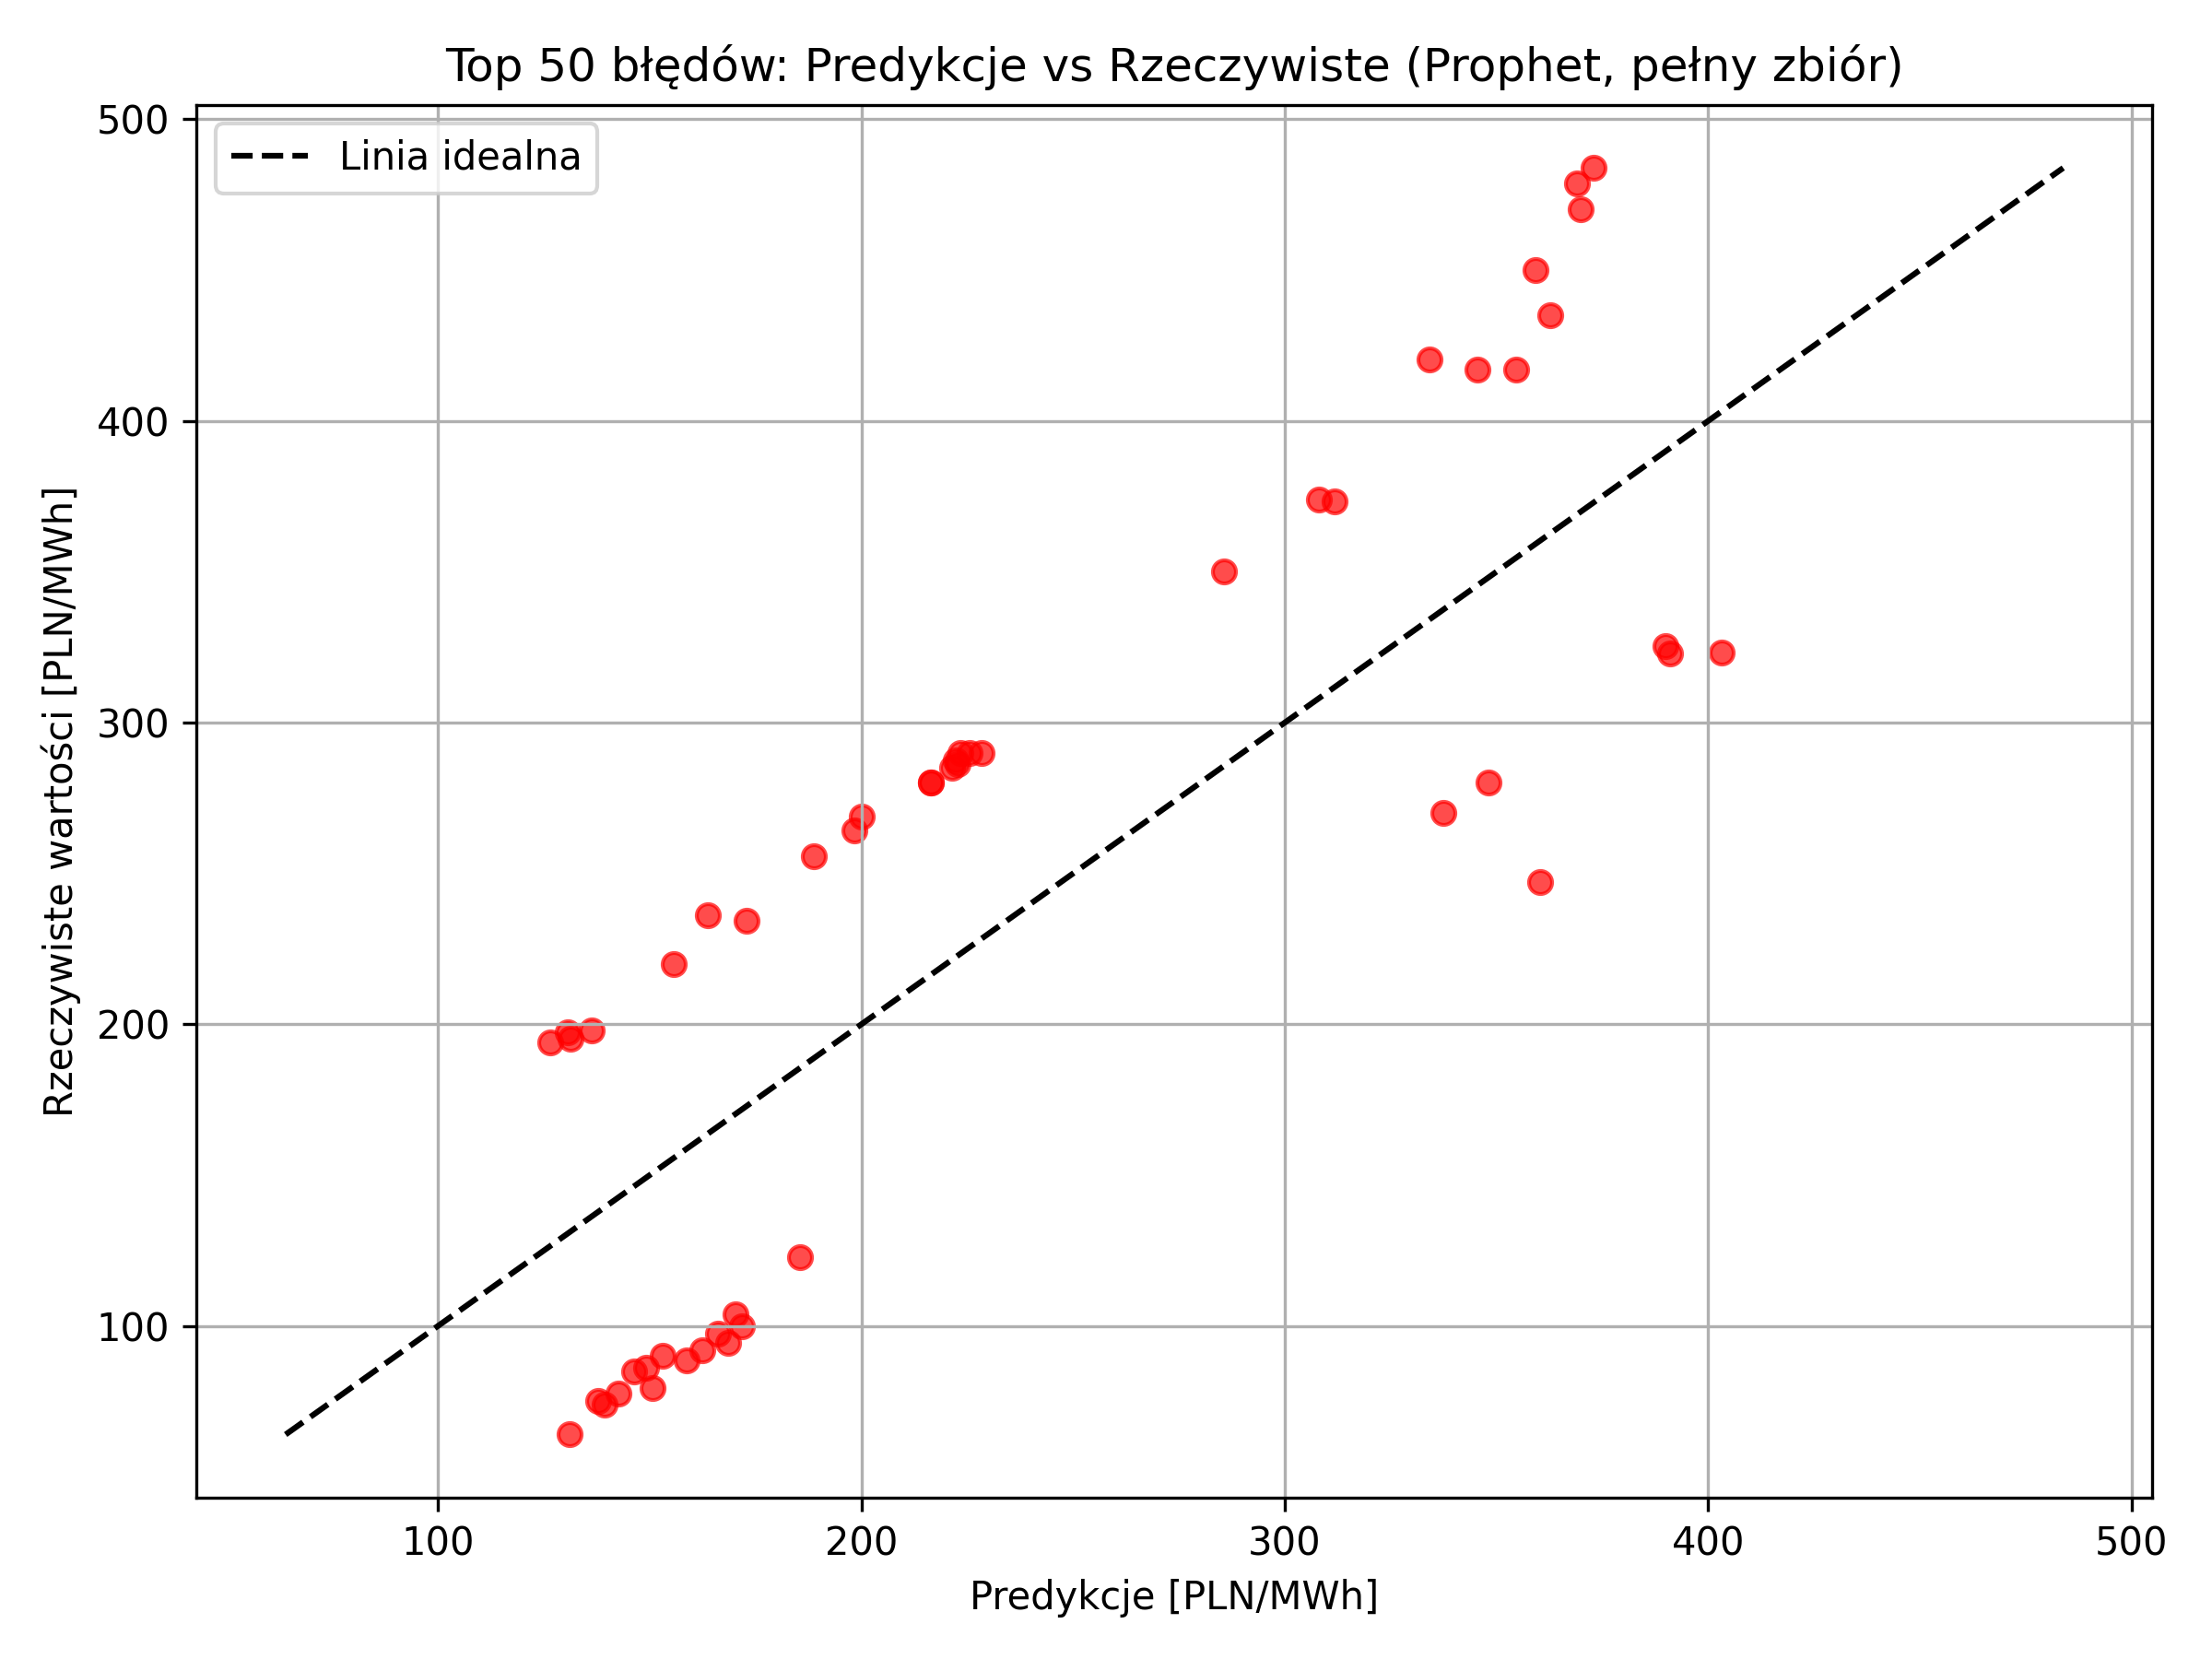
\includegraphics[width=1.0\textwidth]{../plots/predicts/top_50_errors_Prophet_full_stable_period.png}
    \caption{Największe błędy prognoz modelu Prophet z okresu stabilnego. Opracowanie własne.}
    \label{fig:top_50_errors_Prophet_full_stable_period}
\end{figure}

\section{Podsumowanie}
\label{sec:podsumowanie}

Niniejsza praca magisterska koncentrowała się na przygotowaniu i analizie obszernego zbioru danych na potrzeby prognozowania cen energii elektrycznej na Rynku Dnia Następnego w Polsce. Głównym celem było zgromadzenie danych obejmujących lata 2016-2023, które odzwierciedlałyby zarówno okresy stabilności cenowej, jak i momenty wysokiej zmienności spowodowane czynnikami ekonomicznymi, geopolitycznymi i pogodowymi. Udało się stworzyć kompleksową bazę danych zawierającą wiele zmiennych, wpływ których na ceny energii potwierdzają wyniki wybranych modeli, analiza korelacji oraz literatura analizująca rynki zagraniczne.

Wyniki badań wskazują, że przygotowany zbiór danych jest wartościowy i pozwala na budowę modeli o zadowalającej jakości predykcji, szczególnie w okresie stabilnym. Modele statystyczne, takie jak regresja Ridge, okazały się być solidnym i efektywnym podejściem. Model Prophet również dostarczył konkurencyjnych prognoz, zwłaszcza w okresie niestabilnym, podkreślając swoją zdolność do adaptacji do zmieniających się wzorców sezonowych i trendów przy odpowiednim doborze hiperparametrów. Model MLP, mimo potencjału do modelowania złożonych nieliniowości, nie wykazał w tym badaniu jednoznacznej przewagi, a jego wyniki były silnie zależne od doboru cech i warunków rynkowych, co sugeruje konieczność dalszych badań nad optymalizacją jego architektury i procesu uczenia dla tego konkretnego zadania.

Praca potwierdziła trudności związane z prognozowaniem cen energii w warunkach wysokiej zmienności rynkowej, jakie miały miejsce w latach 2020-2023. Wszystkie modele wykazywały wyższe błędy prognoz w tym okresie, co podkreśla wyzwania związane z wpływem nieoczekiwanych czynników zewnętrznych i nieliniowością danych.

Opracowany zbiór danych oraz przeprowadzone analizy mogą stanowić cenne źródło informacji dla uczestników rynku energii w podejmowaniu decyzji handlowych i zarządzaniu ryzykiem. Dalsze kierunki badań mogłyby obejmować eksplorację bardziej zaawansowanych metod uczenia maszynowego, w tym podejść hybrydowych łączących różne techniki modelowania, a także analizę wpływu dodatkowych czynników, takich jak nastroje rynkowe czy zmiany regulacyjne. Istotne byłoby również zbadanie metod radzenia sobie z ekstremalnymi wartościami cen i skokami, które stanowią największe wyzwanie dla modeli prognostycznych.
